% THIS IS A LATEX TEMPLATE FILE FOR PAPERS INCLUDED IN THE
% *Anthology of Computers and the Humanities*. ADD THE OPTION
% 'final' WHEN CREATING THE FINAL VERSION OF THE PAPER. 
% DO NOT change the documentclass
%\documentclass[final]{anthology-ch} % for the final version
\documentclass{anthology-ch}         % for the submission

% LOAD LaTeX PACKAGES
\usepackage{booktabs}
\usepackage{graphicx}
% ADD your own packages using \usepackage{}

% TITLE OF THE SUBMISSION
% Change this to the name of your submission
\title{Seeing History Unseen: Evaluating Vision-Language Models for WCAG-Compliant Alt-Text in Digital Heritage Collections}

% AUTHOR AND AFFILIATION INFORMATION
% For each author, include a new call to the \author command, with
% the numbers in brackets indicating the associated affiliations 
% (next section) and ORCID-ID for each author.  
\author[2,1]{Moritz Mähr}[
  orcid=0000-0002-1367-1618
]

\author[1]{Moritz Twente}[
  orcid=0009-0005-7187-9774
]

% There should be one call to \affiliation for each affiliation of
% the authors. Multiple affiliations can be given to each author
% and an affiliation can be given to multiple authors. 
\affiliation{1}{University of Basel}
\affiliation{2}{University of Bern}

% KEYWORDS
% Provide one or more keywords or key phrases seperated by commas
% using the following command
\keywords{alt-text, vision-language models, accessibility, WCAG 2.2, digital heritage collections, historical accuracy, human-in-the-loop, ethical implications, metadata, disability justice}

% METADATA FOR THE PUBLICATION
% This will be filled in when the document is published; the values can
% be kept as their defaults when the file is submitted
\pubyear{2025}
\pubvolume{1}
\pagestart{1}
\pageend{1}
\conferencename{Proceedings of Conference XXX}
\conferenceeditors{Editor1 Editor2}
\doi{00000/00000}  

\addbibresource{bibliography.bib}

%%%%%%%%%%%%%%%%%%%%%%%%%%%%%%%%%%%%%%%%%%%%%%%%%%%%%%%%%%%%%%%%%%%%%%%%%%%
% HERE IS THE START OF THE TEXT
\begin{document}

\maketitle

\begin{abstract}
Digital archives promised to democratize access to cultural heritage, yet a significant portion of visual historical content remains inaccessible to blind and low-vision readers. This short paper explores the feasibility, accuracy, and ethics of using state-of-the-art vision-language models to generate WCAG-compliant alt-text for a heterogeneous digital heritage collection. We combine computational experiments with qualitative evaluation to develop a framework for responsible AI-assisted accessibility in the humanities.
\end{abstract}

\section{Introduction}

Digital archives promised to democratize access to cultural heritage, yet a significant portion of visual historical content remains inaccessible to blind and low-vision readers. Many digitized photographs, maps, manuscripts, and other images lack descriptive alternative text (alt-text), creating an epistemic barrier to the past. This perpetuates an asymmetry in sensory access to history, where sighted people hold privileged insight into visual sources while others are excluded. Making images legible through text is more than a technical fix---it is a matter of historical justice and inclusivity in digital humanities. Even beyond vision-impaired users, rich image descriptions can aid others, such as neurodivergent readers who benefit from explicit detail that sighted users might glean implicitly \autocite{cecilia2023b}.

Alt-text itself is not new: the HTML \texttt{alt} attribute dates back to the 1990s to support accessibility. However, providing high-quality image descriptions has often been a secondary priority in scholarly communication \autocite{cecilia2023a}. Crafting alt-text is labor-intensive and typically left to authors or curators as a final step, if done at all. As Conrad \autocite{conrad2021} observes, the burden falls on sighted experts to determine what information \emph{is} or \emph{is not} included in an image’s description, an ethical responsibility that only the content’s author can fully shoulder. Author-generated descriptions are valued for capturing contextual meaning that automated tools might miss. They can greatly enhance the accessibility, searchability, and archivability of digital scholarship. Yet in practice, many projects---especially smaller public history initiatives---lack the resources to implement accessibility from the start. The result is that visual evidence remains ``unseen'' by those who rely on assistive technologies.

Recent advances in multimodal AI offer a potential remedy. Vision-Language Models (VLMs) such as OpenAI’s GPT-4o, Google’s Gemini 3, and open-source systems like LLaVA-Next or Mistral’s Pixtral now claim near-human performance in image description tasks. These models can ingest an image and generate a caption or description, essentially simulating the interpretive act of a human describer. If guided properly, such models could produce high-quality, historically informed, and Web Content Accessibility Guidelines (WCAG 2.2)–conformant alt-text. This would dramatically reduce the human effort required to remediate large collections, enabling heritage institutions to scale up accessibility by generating alt-text for thousands of images. In turn, the ``readership'' of digital archives would expand to include those previously left out.

However, adopting automated captioning in a heritage context raises critical questions about truth, evidence, and authenticity. Delegating descriptive labor to machines is not a neutral technical fix; it is an act imbued with values and biases. Deciding what details to include in an image’s description is technically difficult and ethically fraught, especially for historical images depicting people or sensitive cultural content. Vision models trained on general web images may inject anachronistic terms or biases (e.g., misidentifying a 1920s street scene as ``Victorian''), reinforce curatorial blind spots, or omit crucial context that a human historian would provide. There is also the danger of \emph{techno-ableism} \autocite{shew2023}, where blind users’ needs are superficially addressed by technology without truly empowering them or respecting their perspectives. Uncritical use of AI could inadvertently recentre the sighted, algorithmic point of view rather than the lived experience of those using the alt-text.

In this work, we argue that AI-generated alt-text for historical collections is a pivotal test case for the entanglement of AI innovation, archival practice, and disability justice. But can a machine ``see'' history as we do? If a model can convincingly describe a photograph from 100 years ago, how does that change the way we verify and trust such descriptions? Embracing this kind of ``machine vision'' in historical scholarship may require new protocols akin to earlier paradigm shifts (for example, the move from handwritten catalog cards to MARC records, or from microfilm to digital scans). Just as those changes demanded critical awareness of how tools shape historical discovery, the use of AI-generated descriptions demands a new hermeneutic of suspicion. We must learn to critically read machine-generated metadata, much as we read any human-produced finding aid or annotation \autocite{fickers2022}.

The central purpose of our study is to assess whether and how current AI models can serve as \emph{accessibility assistants} in a digital history workflow, and to develop a critical framework for using them responsibly. Our approach is interdisciplinary, blending computational experimentation with qualitative, historiographically informed analysis. Concretely, we plan to experiment with state-of-the-art multimodal models to generate alt-text for a real-world public history collection, and we will evaluate the results for accessibility compliance, historical accuracy, and ethical soundness. By doing so, we aim to illuminate both the opportunities and the pitfalls of integrating AI into inclusive humanities scholarship. Each AI-generated caption is treated not just as metadata but as an interpretive act---one that can be scrutinized like any primary source.

To guide this inquiry, we pose the following research questions:

\begin{enumerate}
    \item \textbf{Feasibility:} \emph{Can current vision-language models produce useful, WCAG 2.2–compliant alt-text for complex historical images when provided with contextual metadata?} We will examine whether models can meet accessibility guidelines (providing text alternatives that convey the same information as the image) and how the inclusion of metadata influences their output. We also consider the potential usefulness of these descriptions for both blind users and sighted users who may benefit from clear explanatory captions \autocite{cecilia2023b}.
    \item \textbf{Quality and Authenticity:} \emph{How do domain experts (e.g., historians) rate AI-generated image descriptions in terms of factual accuracy, completeness, and usefulness for understanding historical content?} We will evaluate the outputs for errors such as anachronisms, misidentifications, or hallucinated details, checking them against known facts from metadata and expert knowledge.
    \item \textbf{Ethics and Governance:} \emph{What are the ethical implications of using AI to generate alt-text in heritage collections, and what human oversight or policy safeguards are required for responsible use?} We will identify potential harms such as biased descriptions (e.g., normative terms), and address the broader question of how much interpretive agency should be ceded to AI in a curatorial context. We will explore strategies to mitigate these risks, including human-in-the-loop editing and transparency measures.
\end{enumerate}

By answering these questions, our work will provide an empirical baseline for \emph{AI-assisted accessibility in the humanities}. It will also offer a reflective critique, examining AI outputs as objects of study in their own right. In the following sections, we outline our data and methodology (Section 2), present initial observations from our experiments (Section 3), and discuss implications for digital humanities practice (Section 4), before concluding with planned next steps (Section 5).

\section{Data: The \textit{Stadt.Geschichte.Basel} Collection}

To ground our evaluation in a real-world scenario, we use the digital collection of the public history project \emph{Stadt.Geschichte.Basel} (an open research repository on the history of Basel, Switzerland). The collection in its final form comprises approximately 1,500 heterogeneous digitized items, including historical photographs, reproductions of artifacts, city maps and architectural plans, handwritten letters and manuscripts, statistical charts, and printed ephemera (e.g., newspaper clippings, posters). Each item is accompanied by metadata in a Dublin Core schema (including fields such as title, creator, date, location, and a descriptive summary provided by historians). Crucially, none of the items currently have alt-text for use with screen readers, making this an ideal testbed for our study. The diversity of the corpus poses a significant challenge to automated captioning: many images are visually and historically complex, requiring domain knowledge to describe properly. This dataset thus allows us to investigate whether AI captioners can handle the ``long tail'' of content found in historical archives, beyond the everyday photographs on which many models are trained.

For our experiments, we have obtained the collection images (in JPEG format, at a standardized size of $\sim$800$\times$800 pixels for computational efficiency) and their corresponding metadata in JSON format. We construct a working dataset where each entry consists of an image and its metadata (e.g., title, date, description). This metadata will be used to prompt the models, as described below. We intend to release the dataset of images, metadata, and model-generated descriptions as a benchmark for future research, following the conference’s emphasis on open data and reproducibility.

\section{Methodology}

Our approach combines a technical pipeline for generating candidate alt-text with a multi-layered evaluation strategy. A human-in-the-loop process is incorporated throughout to ensure quality control and address ethical considerations.

\begin{figure}[ht]
    \centering
    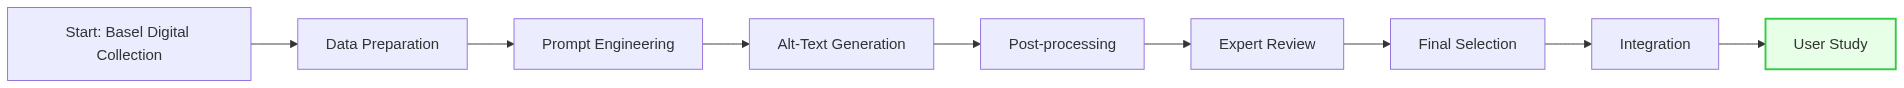
\includegraphics[width=0.8\textwidth]{figure1.png}
    \caption{Alt-text generation and evaluation pipeline.}
\end{figure}

In this short paper, we describe the methodology in future tense, as several steps are in progress.

\subsection{Alt-Text Generation Pipeline}

\textbf{Model Selection:} We have selected four state-of-the-art vision-language models (as of mid-2025) to generate image descriptions. These represent a mix of proprietary and open-source systems: (1) \textbf{GPT-4o} (OpenAI’s multimodal GPT-4o), (2) \textbf{Google Gemini (Vision)}, (3) \textbf{LLaVA-Next} (an open-source vision-LLM based on LLaMA-2, fine-tuned for vision-chat tasks), and (4) \textbf{Mistral Pixtral} (a vision-language model from Mistral’s NeMo framework). We include multiple models to gauge the range of performance and to see how open models compare to the cutting-edge commercial systems. All models are capable of accepting image input and returning a text description. Where possible, we use the latest available model checkpoints or API versions.

\textbf{Prompt Design:} A key feature of our pipeline is providing each model with contextual metadata alongside the image, in order to ground the generation in relevant historical facts. We designed a prompt template (in the same language as the collection, i.e., German) that injects structured metadata fields and instructs the model to follow best practices for alt-text. In essence, the prompt tells the model that it is an \textbf{accessibility assistant} tasked with producing an alt-text for a cultural heritage image. It includes guidelines drawn from the WCAG 2.2 and accessibility literature on how to write good alt-text. For example, the prompt directs the model not to start with redundant phrases like ``Bild von\ldots'' (``image of\ldots''), to be concise (typically under $\sim$120 characters for a simple informative image), and to include any essential visual text (like signs or captions visible in the image). It also asks the model to identify the type of image and adjust the response accordingly: e.g., if the image is a complex diagram or map, the model should produce a short alt-text plus note that a longer description will be provided; if the image is merely a photograph with informative content, a 1--2 sentence description suffices; if the image is mainly text (say a scanned document or poster), the model should either transcribe it (for short text like a sign) or indicate that a full transcription is available elsewhere for longer texts. These rules were distilled from accessibility resources \autocite{a11ychecklist,wcag2023} to ensure the output serves blind users properly. An example snippet of our prompt template is: \emph{``You are an expert in writing WCAG-compliant alt-text. The image comes from a history archive with metadata. Read the metadata and analyze the image. Determine the image type (informative photo, complex diagram/map, or text image) and produce the appropriate alt-text as per the guidelines\ldots''}---followed by the specific instructions for each case. We have found in preliminary trials that including the complete metadata (\texttt{title}, \texttt{date}, etc.) in the prompt can prevent certain errors (for instance, knowing the year of the photo helps the model avoid describing attire as ``modern''). All models are prompted with the same template structure for consistency, and all outputs are requested in German (to match the collection’s context and end-user language).

\textbf{Generation and Post-processing:} Using this prompt, we will run each image through each of the five models, yielding up to five candidate descriptions per image. The generation process will be automated via a Python script (using an API wrapper or library for each model). We anticipate producing around 6,000 candidate alt-texts (4 per image for $\sim$1,500 images). After generation, minimal post-processing will be applied. In particular, we will strip any extraneous phrases if a model fails to follow instructions exactly (e.g., some might prepend ``Alt-Text:'' or polite greetings, which we will remove). We will not otherwise modify the content of the AI outputs at this stage. All results will be stored along with metadata and model identifiers for evaluation.

If a model refuses to describe an image due to some built-in safety filter (misidentifying a historical photograph as sensitive content), we will handle those on a case-by-case basis by leaving that image for human description. Overall, this pipeline is designed to maximize coverage (getting at least one description for every image) while maintaining quality through careful prompting.

\subsection{Evaluation Strategy}

Our evaluation of the AI-generated alt-text will address both \textbf{accessibility compliance} and \textbf{historical accuracy} in line with the research questions. We describe the planned evaluation steps below. All evaluation will be done on a representative subset of the data (approximately 100 images) due to time constraints, with the aim of scaling up later.

\begin{description}
\item[(a) Accessibility and WCAG Compliance:] We will assess whether the AI outputs meet established accessibility guidelines for alt-text. This involves checking each description against a checklist of best practices (e.g., does the alt-text sufficiently describe the image’s important content and function? Does it avoid unnecessary phrases like ``an image of''? If the image contains readable text or numbers, are those included or summarized in the alt-text?). We are adapting the Alt Text Checklist from the A11y Project and WCAG techniques as our evaluation rubric. Each candidate description for an image will be reviewed by at least two team members with knowledge of accessibility standards. In cases where the image is a diagram or chart, we will check that the model followed instructions (providing a short summary alt-text and indicating a longer description would be needed). For images of documents, we check that any text was appropriately handled (transcribed or deferred to full text). The outcome of this step will be a rating or rank of the candidates for each image in terms of compliance. We expect that the model prompted with metadata and guidelines will produce mostly compliant alt-text, whereas some simpler models might yield overly generic or incomplete captions. An initial pilot test supports this: for example, without metadata, an open-source model captioned a photo as ``Old photo of a street'' which misses key specifics, but with our metadata-enhanced prompt GPT-4o produced ``Schwarzweiß-Fotografie einer belebten Straße in Basel, 1917, mit Demonstranten, die Banner in Frakturschrift halten.'' (Black-and-white photograph of a busy Basel street in 1917, with protesters holding banners in Gothic script), which is far richer and ticks more of the accessibility boxes (it mentions the context, the presence of text on banners, etc.). This step addresses the first research question by testing whether models can be guided to meet alt-text requirements. We will quantify common compliance issues and note which model outputs most often require correction.

\item[(b) Historical Accuracy and Usefulness:] The second layer of evaluation focuses on the content accuracy and value of the descriptions from a historian’s perspective. We will conduct a blind review where domain experts (trained historians) examine the AI-generated alt-text for a given image and compare it to the known metadata or facts about that image. Each expert will be presented with the four alt-text candidates for an image and will be asked to order them by relative factual correctness---that is, ranking the descriptions from most to least accurate in terms of representing the image content. This ranking focuses on the relative quality among the alternatives rather than absolute judgments. For example, a model might mistakenly label a horse-drawn carriage in a 1890 photo as a ``car'' (anachronistic), or it might hallucinate a ``red stamp in the corner'' of a document that does not exist. Such errors are critical to catch, as they could mislead researchers. On the other hand, we will also note cases where the AI description includes details that the original metadata or caption did not mention. In preliminary tests, we observed instances of this ``AI insight'': e.g., a model noted ``ein handgezeichneter roter Umriss auf dem Stadtplan'' (a hand-drawn red outline on the map) which the human catalog description had not recorded. Upon checking the image, there was indeed a red pen marking on the map, presumably added by a later hand. Discovering these additional details could be beneficial, pointing scholars to visual evidence they might otherwise overlook. Our expert reviewers will differentiate between such legitimate additions and illegitimate hallucinations. We aim to categorize common error types (misidentifications, missed context, invented details) and measure the proportion of AI-generated alt-text that is acceptable with minimal or no editing versus those that need substantial correction. We anticipate, based on prior work and initial runs, that a majority of descriptions (over 90\%) will be largely correct, while a significant minority will have issues requiring human intervention. The results of this step will inform how much post-editing effort is needed when deploying these models in practice.

\item[(c) Ethical Review:] In parallel with the above, we will perform a qualitative analysis of the AI outputs to identify any ethical or bias concerns. This involves scanning the descriptions for inappropriate language or perspective. For instance, we will check if any descriptions contain terms or tones that are outdated or offensive (e.g., describing people in a demeaning way). We are particularly attentive to \emph{ableist language}: while unlikely, we want to ensure the alt-text does not include phrases like ``suffers from blindness'' or similar, which are not acceptable in modern accessibility writing \autocite{holmes2020}. If the model describes people, we examine whether it is making unwarranted assumptions about their identity (race, gender, etc.) or appearance. One concrete example: one model output described an older photograph of a man as ``ein afrikanischer Mann'' (``an African man''). The image indeed depicted a Black man, but in context his nationality or ethnicity was not documented and not necessarily relevant to the image’s purpose. Including such a descriptor could be seen as othering or speculative, so our policy is to avoid it unless it is directly pertinent \autocite{hanley2021}. In our review process, any such cases will be flagged and either removed or revised. We will also consider the implications of the model’s choices of detail: what the AI focuses on can reflect implicit bias (e.g., always mentioning a woman’s appearance but not a man’s). By compiling these observations, we will derive guidelines for curators on how to handle AI-generated descriptions. The ethical review is not a separate step per se, but integrated into the human-in-the-loop oversight---no AI-generated alt-text will be added to the public collection without passing this human review stage.
\end{description}

\section{Preliminary Results and Observations}

\emph{Note: As this is a work in progress, we report here on initial observations from our ongoing experiments. A full evaluation with quantitative results will be included in the final version.}

\textbf{Feasibility and Throughput:} Early results confirm that using VLMs can dramatically accelerate the production of alt-text for large collections. Our automated pipeline has been able to generate descriptions for the entire set of $\sim$1,500 images in a matter of hours (wall-clock time), only limited by API call rates. In contrast, writing high-quality alt-text manually for that many images would likely take a dedicated team several weeks. Even accounting for time spent in human review and correction, the AI-assisted workflow promises to be far more efficient. Importantly, the models attempted to describe every image; none of the images were outright un-captionable by the AI. Only a small fraction of outputs came back empty or with an error (for instance, a few instances where a model refused output thinking a historical war photo was violent content). This suggests that an automated approach can achieve close to near 100\% \emph{coverage}, ensuring that no image remains without at least an initial draft description. From an accessibility standpoint, this is already a win: having even a basic description is better than nothing for a user navigating these archives.

\textbf{Alt-Text Quality --- Accuracy vs.\ Errors:} The quality of the AI-generated descriptions varies across models and images, but our expert review so far indicates a majority are quite descriptive and useful, with some requiring only minor tweaking. For straightforward photographs (e.g., a city street, a portrait, an artifact on a plain background), the models often produced accurate and succinct descriptions. In many cases, the AI caption actually included more concrete detail than the existing human metadata. For example, one image of a tram scene had a human description ``Street scene with tram and people, Basel early 1900s.'' A model-generated alt-text added detail: ``Drei Männer stehen vor einem Straßenbahnwagen. Der mittlere Mann hält ein Schild mit der Nummer 5.'' (Three men stand in front of a tram car. The middle man is holding a sign with the number 5.) Such details can enrich the record and provide a fuller picture to someone who cannot see the image. This demonstrates the potential for AI to surface elements that a human might overlook or assume as understood.

At the same time, we have observed a number of \emph{failure modes} that reinforce the need for human oversight. A preliminary categorization of issues includes: \textbf{Hallucinated Details:} Occasionally the model introduces objects or readings that are not actually present. For instance, one caption described ``an official seal stamped on the document'' when no such seal exists on the image. Another described ornate architectural details on a building that were in reality not discernible. \textbf{Anachronisms and Misidentifications:} Some outputs used terms that were out-of-place for the historical context. We saw an example of a model calling a 1910 protest scene ``Victorian''---confusing the era.

\textbf{Model Comparisons:} A full benchmarking is ongoing.

\textbf{Ethical and Sensitive Cases:} Our review of outputs is ongoing, but so far we have not encountered any egregiously biased or harmful descriptions from the models when they are properly prompted. This is a relief given past incidents in vision AI (for example, earlier algorithms infamously mis-labelled images of Black people with animal names, as noted by Hanley et al. \autocite{hanley2021}). None of our models produced derogatory labels or inappropriate descriptions of people; they generally stuck to neutral terms like ``an older woman,'' ``a young boy,'' etc., only mentioning apparent race or disability if it was obvious and relevant (which we typically consider outside the scope of alt-text unless the historical context makes it pertinent). We also noted that models occasionally avoided describing graphic historical images in detail when the content was discriminatory. In those cases, a human will likely need to step in to provide an appropriate description that the AI hesitated to give.

Overall, our preliminary findings suggest that with careful prompting and human curation, AI-generated alt-text can achieve a quality that makes them valuable for accessibility in digital heritage collections. The process is \textbf{feasible} and scalable (addressing the first research question), and the outputs are often accurate and informative, though not without errors (addressing the second research question). Importantly, this exercise has started to reveal where AI captions might \emph{add} value (by noticing visual details) and where they might \emph{mislead} (by hallucinating or omitting context). These insights will feed into the development of guidelines and best practices for using AI in this capacity.

\section{Discussion and Future Work}

Our ongoing project highlights both the promise and the complexities of integrating AI into cultural heritage accessibility. Here we reflect on key implications and outline the next steps, including a planned user study and considerations for ethical deployment (addressing the third research question and beyond).

\textbf{Integrating AI into Digital Humanities Practice:} Embracing AI for alt-text generation can substantially improve the inclusivity of digital archives. For public history initiatives, this means that no part of the historical record should remain off-limits to blind or visually impaired researchers. By leveraging AI, even small teams can now consider providing descriptions for thousands of images, bridging an accessibility gap that has persisted in the field. This is a concrete way in which computational methods can democratize access to cultural heritage. However, our work also underscores that AI is not a plug-and-play solution: it requires thoughtful integration. Historians and archivists must develop a new form of source criticism for AI-generated content. Just as we critically evaluate a human-written caption or a transcribed document, we need to critically interrogate AI outputs---asking how the description was generated, what might be missing or biased, and how it should be interpreted. This aligns with the notion of \emph{digital hermeneutics} in public history \autocite{fickers2022}, where scholars maintain a reflexive awareness of the tools mediating their understanding of sources. In practice, this could mean training archival staff in basic AI literacy or establishing review protocols that treat AI suggestions as starting points subject to scholarly validation.

\textbf{Human-AI Collaboration Workflow:} Based on our experiences, we advocate for a workflow where AI assists but humans remain in control of the final output. In our case, the AI handles the first draft generation at scale, and human experts perform targeted reviews and corrections. This collaboration can yield high-quality results while significantly reducing the workload. A crucial part of this workflow is documentation and transparency: we are keeping logs of how each alt-text was generated (which model, what prompt, any edits) so that there is a clear provenance. In the context of GLAM (Galleries, Libraries, Archives, Museums) institutions, such transparency is important for accountability. Users of the archive should be able to tell if a description was AI-generated or curator-written. In our future interface for the \emph{Stadt.Geschichte.Basel} collection, we plan to tag AI-generated descriptions (after they’ve been vetted) with an indication like ``AI-assisted description'' in the metadata. This way, if a user spots an error or has a question, they know that the description is a product of an algorithmic process and can flag it for review.

\textbf{Ethical Considerations:} Deploying AI in heritage description brings several ethical dilemmas to navigate. One is deciding how to handle sensitive content. We encountered images containing derogatory historical texts (e.g., racist slogans on a 1920s poster). Simply omitting these details would whitewash history, but describing them verbatim could be distressing or violate content guidelines. Our solution will be to include a neutral note in the description (e.g., ``poster with discriminatory slogan (not quoted here)'') and ensure a full transcription is available on request or in a separate text. Another dilemma is the balance between description and interpretation. Alt-text guidelines advise objectivity, but in historical collections, a certain level of interpretation (identifying the context or significance) can greatly enhance comprehension. We have leaned towards \emph{describing with context}---for instance, identifying a person by their role if known (``the Mayor of Basel'') rather than just ``a man,'' or noting the event if it’s documented. We argue that this approach respects the spirit of alt-text (to convey the same information sighted viewers get, which often includes context from captions or exhibit labels). Nonetheless, we refrain from speculation: the AI might guess emotions or motivations (``appears angry'')---we do not include such unverified interpretations in the final alt-text.

\textbf{Toward Guidelines and Policy:} One outcome of this project will be a set of practical guidelines for heritage institutions considering AI-generated metadata. We are already formulating recommendations such as: always keep a human in the loop as the final decision-maker; establish an internal content style guide for AI to follow (including sensitive language to avoid or preferred terminology); be mindful of copyright (for modern images, an overly detailed description might infringe on the creator’s rights, so in some cases a simpler description might be prudent---although accessibility needs often qualify as fair use in many jurisdictions). In the long term, it may be beneficial to fine-tune or train models on \emph{historical image caption} data to reduce errors---an avenue for future research. For now, prompt engineering and careful curation are our main tools to align general models with the specialized needs of historical content.

\textbf{User Study (Planned):} Ultimately, the success of AI-generated alt-text must be measured by how well it serves the end users. As a next step, we plan to conduct a user study involving two key groups: blind or low-vision individuals who rely on screen readers, and neurodiverse individuals (such as those with dyslexia or certain cognitive disabilities) who benefit from supplemental text descriptions of images. In this study, participants will interact with a selection of images from the collection, accompanied by either human-written or AI-generated alt-text (without knowing which is which). We will evaluate their understanding of the images (through follow-up questions or tasks), the usability of the descriptions (time taken to get information, any confusion or misinterpretation), and gather subjective feedback on satisfaction. This will provide valuable insights into whether the AI-generated descriptions are meeting the needs of real users. For example, a blind user might tell us if the description painted a sufficient mental picture, or a neurodiverse user might comment on whether the alt-text clarified the image in a helpful way. We expect to learn whether our AI-assisted alt-text is truly effective or if there are gaps we didn’t anticipate. The results of this user study will inform further refinement of the alt-text (perhaps prompting us to include more or less detail) and will ground our work in the lived experiences of the people we aim to support.

\section{Conclusion}

In this work-in-progress, we explored the use of multimodal AI models to generate accessible image descriptions for a digital heritage collection. Our initial findings are encouraging: with the right prompts and metadata, models like GPT-4o can produce alt-text that significantly lowers the barrier to making historical images accessible, saving time and labor for human experts. This approach has the potential to transform how digital archives practice accessibility, by ensuring that visual content is not exclusively available to sighted audiences. At the same time, our study highlights important considerations for accuracy and ethics. AI-generated descriptions must be vetted for errors and biases; they should complement, not replace, the discerning eye of the historian or archivist. We have shown that a collaborative human-AI workflow can harness the strengths of both---scale and speed from the AI, contextual judgment from the human---to achieve a result that neither could accomplish alone at this scale.

Moving forward, we will complete our systematic evaluation and user study, and we will refine our methods accordingly. We plan to release the dataset of images, metadata, and model-generated alt-text (with any necessary permissions and safeguards) to serve as a benchmark for others. We also acknowledge that there are open questions regarding intellectual property and privacy when using AI in this manner: for instance, how do we handle detailed descriptions of artworks or personal photographs that are under copyright? Our stance is that providing textual descriptions for accessibility is generally justified (and often legally exempt for assistive purposes), but each institution should develop policies in consultation with legal experts. We will include a brief guideline in our final paper on managing these concerns.

Finally, our work contributes to a larger conversation in computational humanities about the role of AI in research workflows. By treating AI outputs as objects of interpretation and by centering accessibility, we hope to model a thoughtful integration of technology in humanities scholarship. As one participant in our discussions noted, this is about \emph{``making the past accessible in the present, to everyone.''} We believe that is a goal worth pursuing with the combined efforts of historians, technologists, and user communities. We look forward to sharing more complete results soon, and to engaging in dialogue at CHR 2025 on how we can collectively harness AI for inclusive and critical digital heritage practices.


\section*{Acknowledgements}

This unnumbered section should be blank when submitting your paper. After review, you may include lists of people and organizations who supported the work.

% Print the biblography at the end. Keep this line after the main text of your paper, and before an appendix. 
\printbibliography

% You can include an appendix using the following command
% \appendix

% \section{First Appendix Section} \label{appdx:first}

% Appendix sections should be ordered by letters rather than numbers, and their contents do not count towards the paper's length limit. Appendix sections may also contain additional tables and figures.  

\end{document}
